\section{Structure Learning}

\begin{frame}{Challenges in Structure Learning}
\begin{itemize}
    \item The generated structure has to be complete and decomposable, i.e., a sparsely connected graph.
    \item We are interested in structures that generalise well, many approaches learn deep trees that are prune to overfit.
    \item Until recently\footnote{\scriptsize M. Trapp et al.: Bayesian learning of sum-product networks. In NeurIPS, 2019.\label{fn:bspn}}, there has been no clear defined goal or principle of what makes a good structure.
\end{itemize}
\end{frame}


\begin{frame}{General-Purpose Learners (Selection)}{}
\begin{itemize}
    \item LearnSPN\footnote{\tiny R. Gens \& P. Domingos: Learning the structure of sum-product networks. In ICML, 2013.} recursively constructs sum nodes using clustering and product nodes using independence test. The resulting SPN is a tree.
    \item ID-SPN\footnote{\tiny A. Rooshenas \& D. Lowd: Learning Sum-Product Networks with Direct and Indirect Variable Interactions. In ICML, 2014.} is a generalisation of LearnSPN with tractable Markov networks as leaves.
    \item RAT-SPN\footnote{\tiny R. Peharz et al.: Random sum-product networks: A simple but effective approach to probabilistic deep learning. In UAI, 2019.} constructs region-graphs (meta-graph over SPNs) with random decompositions.
    \item BSPN\footnotemark[8] learns structures and parameters using Bayesian inference.
\end{itemize}
\end{frame}

%\begin{frame}{Bayesian Structure \& Parameter Learning \small $[$Trapp2019$]$}
%  \begin{itemize}
%    \item For Bayesian structure \& parameter learning of SPNs we assume $\graph$ is a tree-shaped region graph.
%    \pause
%    \item A region graph $\rg$ is a vectorised representation of SPNs and is a connected DAG containing two types of nodes: regions ($\region \in \regions$) and partitions ($\partition \in \partitions$).
%  \end{itemize}
%  \pause
%  \begin{figure}
%  \centering
%  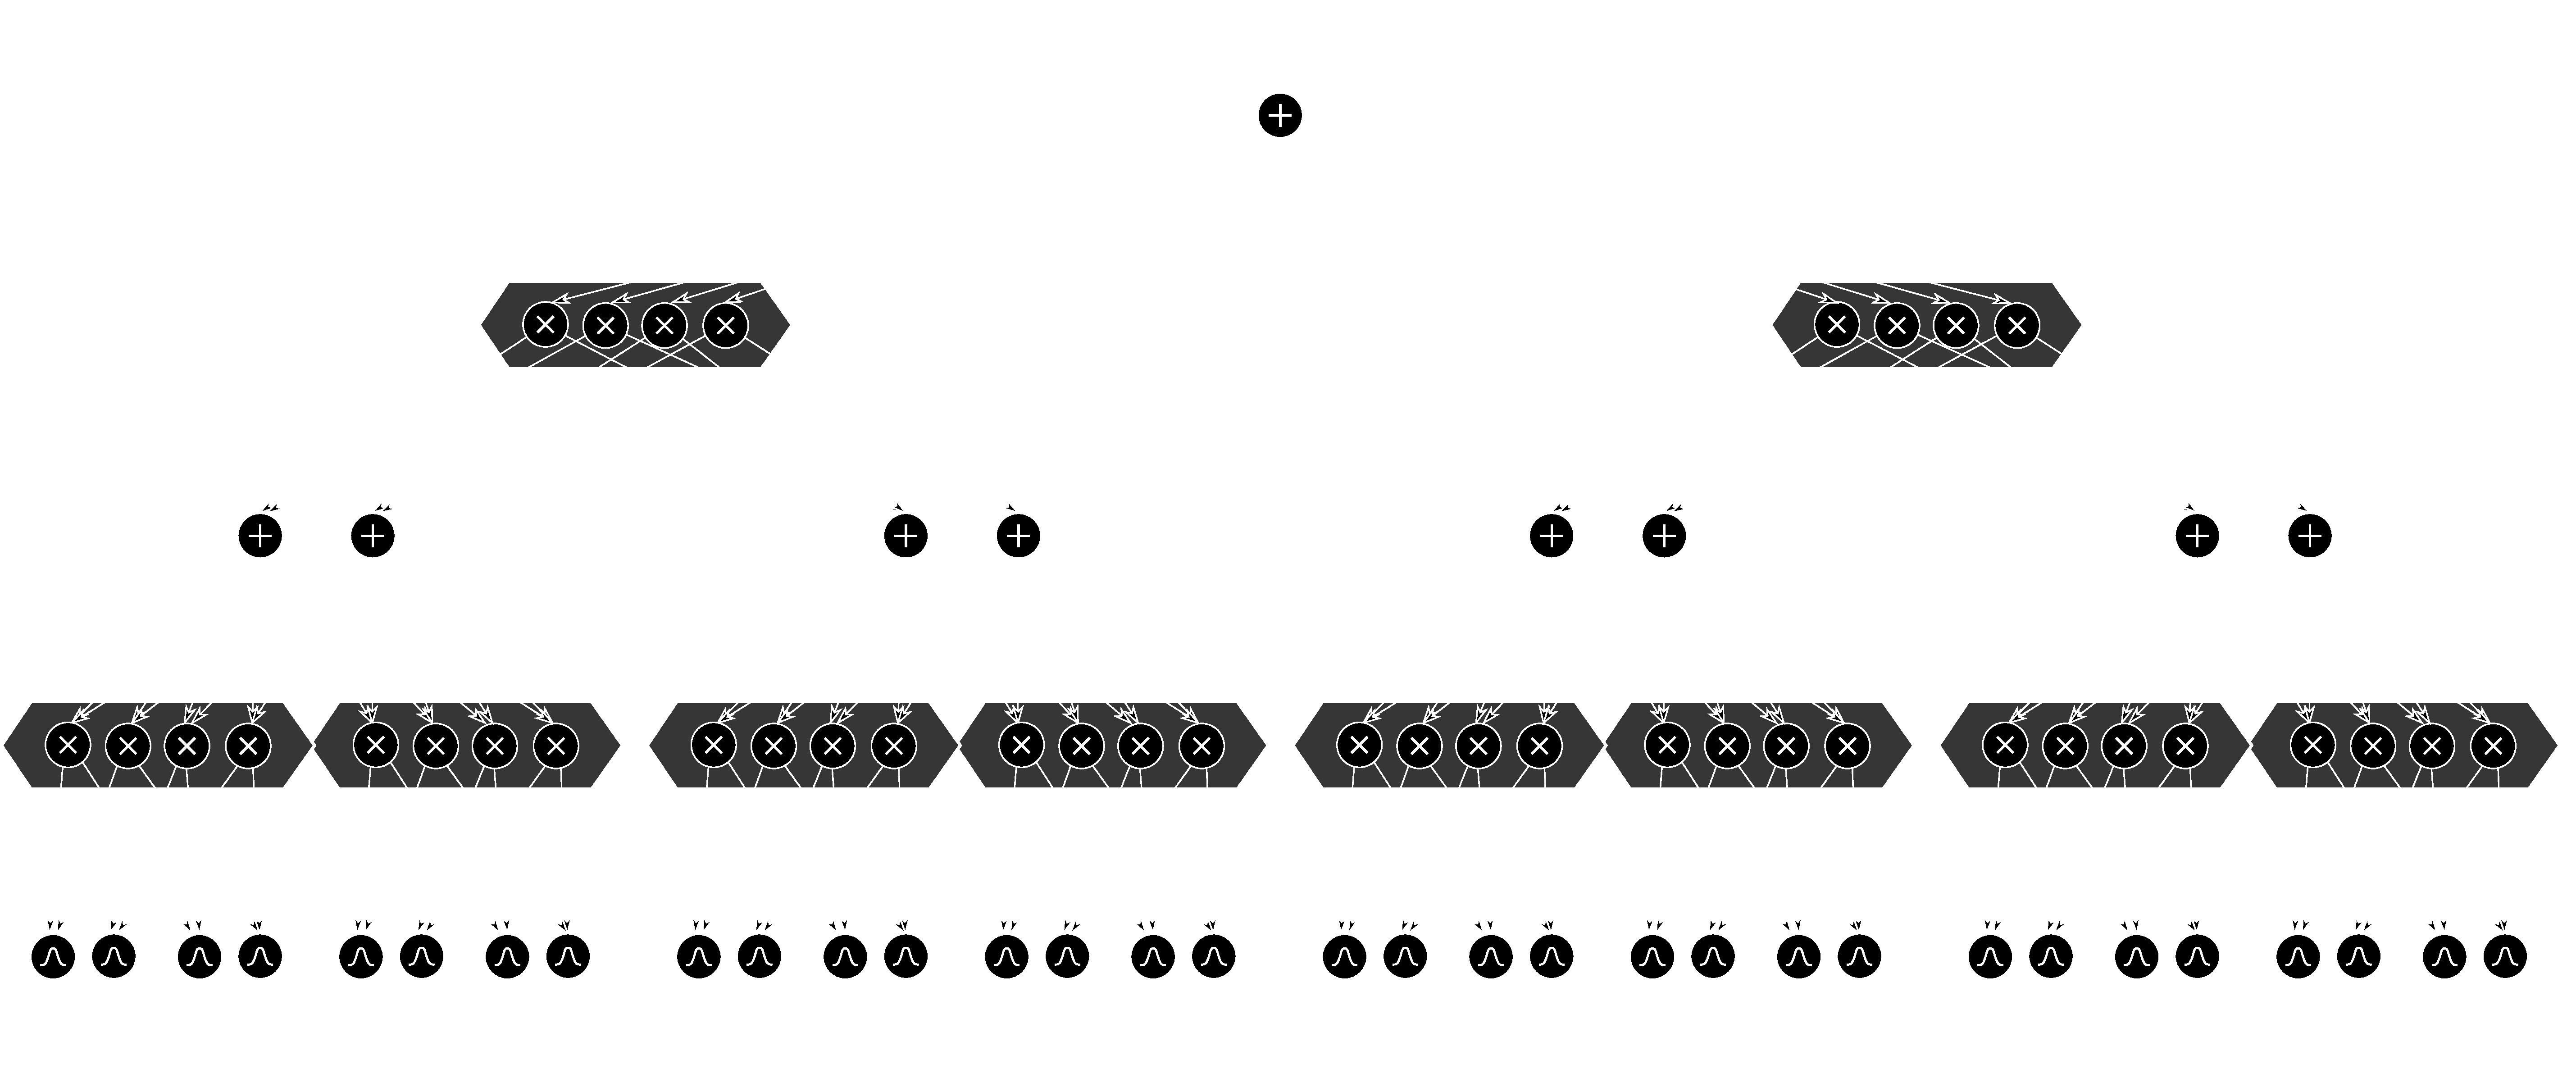
\includegraphics[width=0.9\linewidth]{region-graph}
%  \caption{Example region-graph. Based on the illustration by [Peharz2019].}
%\end{figure}
%
%\end{frame}

\begin{frame}{Bayesian Structure \& Parameter Learning}
\begin{itemize}
    \item We assume $\graph$ is a tree-shaped region graph, i.e., the SPN is a \emph{not} a tree.
    \item For each dimension $d$ we introduce a latent variable $Y_{\partition,d}$ at each partition node (bucket of product nodes).
    \item The latent variables represent an assign of $d$ to a child, given a unique path leading to the node.
\end{itemize}

\begin{figure}
    \centering
    \begin{tikzpicture}
        \node[obs] (x) {$\xnd$};
        \node[latent, left=of x] (z) {$z_{\SumNode,n}$};
        \node[latent, right=of x] (y) {$y_{\partition,d}$};
        \node[latent, below=of y] (t) {$\theta_{\Leaf,d}$};
        \node[latent, below=of z] (w) {$w_{\SumNode}$};
        \node[latent, right=of y] (o) {$\vp_{\partition}$};

        \edge {z,t} {x} ; %
        \edge {y} {x} ; %
        \edge {w} {z} ; %
        \edge {o} {y} ; %

        \plate {zs} {(z)(w)} {$\forall \SumNode \in \SumNodes$} ;
        \plate {yo} {(y)(o)} {$\forall \partition \in \partitions$} ;
        \plate {t} {(t)} {$\forall \Leaf \in \Leaves$} ;
        \plate [inner xsep=0.3cm] {xyt} {(x)(y)(t)} {$d\!\in\!1\!:\!D$} ;
        \plate [inner xsep=0.3cm] {xz} {(x)(z)(xyt.north west)} {$n\!\in\!1\!:\!N$} ;
    \end{tikzpicture}
    \caption{Generative model for Bayesian structure and parameter learning.}\label{fig:BSPN}
\end{figure}
\end{frame}

\begin{frame}{Bayesian Structure \& Parameter Learning}
    \begin{itemize}
        \item Posterior inference can be performed using ancestral within Gibbs sampling.
        \item Bayesian structure learning obtains competitive results on benchmark datasets.
        \item We show that Bayesian SPNs can also be used in heterogeneous data domains and can be extended to nonparametric formulations, allowing principled online learning.
        \item Further, our approach is the only method that can consistently learn under missing data.
    \end{itemize}
\end{frame}


%
%\begin{frame}{Experiments}
% \begin{itemize}
%    \item We compared the performance of our approach against SOTA structure learners on discrete, heterogeneous and data with missing values.
%    \pause
%    \item The discrete datasets are standard benchmark datasets.
%    \pause
%    \item We evaluated against an increasing number of observations having $50\%$ dimensions missing completely at random to assess the robustness.
%\end{itemize}
%\pause
%\small Note: Existing approach cannot handle missing data during structure learning, so we either removed the samples with missing data or used k-NN imputation.
%
%\end{frame}
%
%\begin{frame}{Experiments (discrete)}
%  \begin{table}
%
%  \label{tab:discrete}
%
%  \centering
%  \resizebox{0.8\columnwidth}{!}{%
%\begin{tabular}{l*{6}{r}|r}
%
%\toprule
%
%Dataset & LearnSPN & RAT-SPN & CCCP & ID-SPN & ours & ours$^\infty$ & BTD \\
%
%\midrule
%
%NLTCS & $-6.11$ & $-6.01$ & $-6.03$ & $-6.02$ & $\textcolor{CBYellow}{-6.00}$ & $-6.02$ & $-5.97$\\
%
%MSNBC & $-6.11$ & $-6.04$ & $-6.05$ & $-6.04$ & $-6.06$ & $\textcolor{CBYellow}{-6.03}$ & $-6.03$\\
%
%KDD & $-2.18$ & $-2.13$ & $-2.13$ & $-2.13$ & $\textcolor{CBYellow}{-2.12}$ & $-2.13$ & $-2.11$\\
%
%Plants & $-12.98$ & $-13.44$ & $-12.87$ & $\textcolor{CBYellow}{-12.54}$ & \ul{$-12.68$} & \ul{$-12.94$} & $-11.84$\\
%
%Audio & $-40.50$ & $-39.96$ & $-40.02$ & $-39.79$ & \ul{$\textcolor{CBYellow}{-39.77}$} & \ul{$-39.79$} & $-39.39$\\
%
%Jester & $-53.48$ & $-52.97$ & $-52.88$ & $-52.86$ & \ul{$\textcolor{CBYellow}{-52.42}$} & \ul{$-52.86$} & $-51.29$\\
%
%Netflix & $-57.33$ & $-56.85$ & $-56.78$ & $-56.36$ & $\textcolor{CBYellow}{-56.31}$ & $-56.80$ & $-55.71$\\
%
%Accidents & $-30.04$ & $-35.49$ & $-27.70$ & $\textcolor{CBYellow}{-26.98}$ & \ul{$-34.10$} & \ul{$-33.89$} & $-26.98$\\
%
%Retail & $-11.04$ & $-10.91$ & $-10.92$ & $-10.85$ & $-10.83$ & $\textcolor{CBYellow}{-10.83}$ & $-10.72$\\
%
%Pumsb-star & $-24.78$ & $-32.53$ & $-24.23$ & $\textcolor{CBYellow}{-22.41}$ & \ul{$-31.34$}& \ul{$-31.96$} & $-22.41$\\
%
%DNA & $-82.52$ & $-97.23$ & $-84.92$ & $\textcolor{CBYellow}{-81.21}$ & $-92.95$ & $-92.84$ & $-81.07$\\
%
%Kosarak & $-10.99$ & $-10.89$ & $-10.88$ & $\textcolor{CBYellow}{-10.60}$ & \ul{$-10.74$} & \ul{$-10.77$} & $-10.52$\\
%
%MSWeb & $-10.25$ & $-10.12$ & $-9.97$ & $\textcolor{CBYellow}{-9.73}$ & $-9.88$ & \ul{$-9.89$} & $-9.62$\\
%
%Book & $-35.89$ & $-34.68$ & $-35.01$ & $-34.14$ & $\textcolor{CBYellow}{-34.13}$ & $-34.34$ & $-34.14$\\
%
%EachMovie & $-52.49$ & $-53.63$ & $-52.56$ & $-51.51$ & $-51.66$ & $\textcolor{CBYellow}{-50.94}$ & $-50.34$\\
%
%WebKB & $-158.20$ & $-157.53$ & $-157.49$ & $\textcolor{CBYellow}{-151.84}$ & \ul{$-156.02$} & $-157.33$ & $-149.20$\\
%
%Reuters-52 & $-85.07$ & $-87.37$ & $-84.63$ & $\textcolor{CBYellow}{-83.35}$ & $-84.31$ & $-84.44$ & $-81.87$\\
%
%20 Newsgrp & $-155.93$ & $-152.06$ & $-153.21$ & $\textcolor{CBYellow}{-151.47}$ & $-151.99$ & $-151.95$ & $-151.02$\\
%
%BBC & $-250.69$ & $-252.14$ & $\textcolor{CBYellow}{-248.60}$ & $-248.93$ & $-249.70$ & $-254.69$ & $-229.21$\\
%
%AD & $-19.73$ & $-48.47$ & $-27.20$ & $\textcolor{CBYellow}{-19.05}$ & $-63.80$ & $-63.80$ & $-14.00$\\
%
%\bottomrule
%
%\end{tabular}
%}
%
%\end{table}
%
%\end{frame}
%
%\begin{frame}{Experiments (missing data)}
%\begin{figure}
%  \begin{minipage}{.48\textwidth}
%     \begin{tikzpicture}
%
%\begin{axis}[
%
%    width=5.5cm,
%
%    height=4cm,
%
%    xlabel={\scriptsize{\% obs. with missing values}},
%
%    ylabel={\scriptsize{test log-likelihood}},
%
%    legend pos=south west,
%    legend columns=2,
%    legend style={font=\tiny},
%    legend image post style={scale=0.5},
%    legend style={fill=background, draw=white, fill opacity=0.6, draw opacity=1,text opacity=1},
%    label style={font=\tiny},
%    tick label style={font=\tiny},
%
%    ymajorgrids=true,
%
%    grid style=dashed,
%
%    cycle list name=my black white
%
%]
%
%\addplot coordinates {
%
%    (20, -53.551654150378006)
%
%    (40, -54.421205612626615)
%
%    (60, -55.51437111821264)
%
%    (80, -57.29533673640321)
%
%    };
%
%\addlegendentry{LearnSPN}
%
%
%\addplot coordinates {
%
%    (20, -52.9306308300396)
%
%    (40, -53.669159658525054)
%
%    (60, -53.804286870223166)
%
%    (80, -55.06448194755978)
%
%    };
%
%\addlegendentry{LearnSPN$^\star$}
%
%
%
%\addplot coordinates {
%
%    (20, -52.332443930626056)
%
%    (40, -52.24919890693739)
%
%    (60, -53.824333727580374)
%
%    (80, -55.41192445685279)
%
%    };
%
%\addlegendentry{ID-SPN}
%
%
%\addplot coordinates {
%
%    (20, -51.71630289170897)
%
%    (40, -52.4355408358714)
%
%    (60, -52.30368237732657)
%
%    (80, -53.173612370558374)
%
%    };
%
%\addlegendentry{ID-SPN$^\star$}
%
%\addplot coordinates {
%
%    (20, -51.784)
%
%    (40, -51.997)
%
%    (60, -52.415)
%
%    (80, -52.85)
%
%    };
%
%\addlegendentry{BSPN}
%
%
%\end{axis}
%
%\end{tikzpicture}
%\caption{EachMovie (D: 500, N: 5526)}
%\end{minipage}
%\begin{minipage}{.48\textwidth}
%  \begin{tikzpicture}
%
%\begin{axis}[
%
%    width=5.5cm,
%
%    height=4cm,
%
%    xlabel={\scriptsize{\% obs. with missing values}},
%
%    legend pos=north east,
%
%    ymajorgrids=true,
%
%    grid style=dashed,
%    label style={font=\tiny},
%    tick label style={font=\tiny},
%
%    cycle list name=my black white,
%
%]
%
%\addplot coordinates {
%
%    (20, -161.41130223478262)
%
%    (40, -163.56351684466114)
%
%    (60, -162.96930286251663)
%
%    (80, -168.00941901059738)
%
%    };
%
%\addlegendentry{learnSPN}
%
%
%
%
%\addplot coordinates {
%
%    (20, -161.4285603783307)
%
%    (40, -165.36322925292424)
%
%    (60, -164.87160515320465)
%
%    (80, -164.53405856701238)
%
%    };
%
%\addlegendentry{learnSPN$^\star$}
%
%
%
%\addplot coordinates {
%
%    (20, -152.1845925143198)
%
%    (40, -154.95268171360382)
%
%    (60, -158.58576871121716)
%
%    (80, -165.45426630310263)
%
%    };
%
%\addlegendentry{ID-SPN}
%
%
%\addplot coordinates {
%
%    (20, -152.26143497732696)
%
%    (40, -153.5671636300716)
%
%    (60, -153.5671636300716)
%
%    (80, -157.2684578353222)
%
%    };
%
%\addlegendentry{ID-SPN$^\star$}
%
%\addplot coordinates {
%
%    (20, -157.078)
%
%    (40, -157.876)
%
%    (60, -158.625)
%
%    (80, -159.123)
%
%    };
%
%\addlegendentry{BSPN}
%  \legend{}; % empty the legend so as not to print it
%
%\end{axis}
%
%\end{tikzpicture}
%\caption{WebKB (D: 839, N: 3361)}
%\end{minipage}
%\begin{minipage}{.5\textwidth}
%  \begin{tikzpicture}
%
%\begin{axis}[
%
%    width=5.5cm,
%
%    height=4cm,
%
%    xlabel={\scriptsize{\% obs. with missing values}},
%
%    legend pos=north east,
%
%    ymajorgrids=true,
%
%    grid style=dashed,
%    label style={font=\tiny},
%    tick label style={font=\tiny},
%
%    cycle list name=my black white
%
%]
% 
%
%\addplot coordinates {
%
%    (20, -250.83622675798426)
%
%    (40, -261.1124401206212)
%
%    (60, -266.0005946312015)
%
%    (80, -273.39617177834293)
%
%    };
%
%\addlegendentry{learnSPN}
%
%
%
%\addplot coordinates {
%
%    (20, -284.24099564475125)
%
%    (40, -261.6701870807035)
%
%    (60, -265.4755544697035)
%
%    (80, -297.06332858812755)
%
%    };
%
%\addlegendentry{learnSPN$^\star$}
%
%
%
%\addplot coordinates {
%
%    (20, -250.68554855757577)
%
%    (40, -253.81061585454546)
%
%    (60, -261.81913693030305)
%
%    (80, -272.27580261212125)
%
%    };
%
%\addlegendentry{ID-SPN}
%
%
%
%\addplot coordinates {
%
%    (20, -249.82204944242426)
%
%    (40, -252.33469486666664)
%
%    (60, -254.56216942424243)
%
%    (80, -256.8125317606061)
%
%    };
%
%\addlegendentry{ID-SPN$^\star$}
%
%\addplot coordinates {
%
%    (20, -251.551)
%
%    (40, -254.101)
%
%    (60, -255.551)
%
%    (80, -256.144)
%
%    };
%
%\addlegendentry{BSPN}
%  \legend{}; % empty the legend so as not to print it
%
%\end{axis}
%
%\end{tikzpicture}
%\caption{BBC (D: 1058, N: 1895)}
%\end{minipage}
%\end{figure}
%
%\end{frame}
